\subsection{Population geometry recovers an anatomical hierarchy across regions}

\begin{figure}
    \centering
    
\includegraphics[width=1\textwidth]{content/figures/netrep-journal-figure-4.pdf}
    \caption{\textbf{Regional geometry reflects anatomical hierarchy in mice} \textbf{a.} Illustration of the Allen Brain Observatory dataset, consisting of K = 56 fine-grained subregions of mouse cortex and thalamus (Right) in response to a naturalistic movie (Left). \textbf{b.}  K x K matrix of pairwise shape distances across all subregions. The matrix is further sorted by clusters found using hierarchical clustering (Methods) \textbf{c.} Visualization of b), using MDS and PCA shows subregions cluster together according to anatomy. \textbf{d.} The same analysis in $K = 22$ cortical areas of the IBL Brainwide Map, where each neuron is summarized by the time-varying coefficients of an encoding model for $8$ task and behavioral variables \parencite{posani2026}, and areas are compared without averaging those coefficients across neurons. \textbf{e.} Procrustes distance between two areas against their anatomical connectivity \parencite{harris2019}; each dot is a pair of areas. \textbf{f.} MDS of the resulting dissimilarity matrix, colored by position in the cortical hierarchy. \textbf{g.} Position in the hierarchy predicted from the dissimilarity matrix by ridge regression, holding out one area at a time.}
    \label{fig:allen}
\end{figure}

After establishing our approach in simulated data, we can ask an open question: Does the ubiquity of decodable information across the brain imply that population geometry is correspondingly uniform? We asked this in three datasets, from mice and nonhuman primates, testing the conventional view that representations morph along an anatomical hierarchy from early sensory to higher-order areas. This view has been challenged by recent reports that most task and behavioral variables are decodable from nearly any brain region \parencite{findling2025brain,angelaki2025brain, Lloreda2025,rosen2026distributed}, though it remains unclear whether the joint arrangement of the entire set of variables is also comparable across regions.

% This question requires us to simultaneously compare numerous neural populations (upwards of 50 brain regions), as well as regression and clustering analyses across these large numbers of recordings. The metric properties of shape space, summarized in \cref{eq:metric-space-equivalence,eq:metric-space-symmetry,eq:metric-space-triangle}, are critical to perform such analyses rigorously.

First, we studied population-level activity across $K=55$ fine-grained subregions of mouse cortex and thalamus in data publicly released by the Allen Brain Observatory \parencite{Siegle2021-hs}.
We focused on extracellular electrical recordings (Neuropixels probes) performed while mice viewed a naturalistic movie (Touch of Evil by Welles, O.; , \textit{Fig.} \ref{fig:allen}a).
Spike counts attributed to isolated units were trial-averaged, normalized, and pooled across subjects before categorizing them into $K=55$ populations based on anatomical location defined by the Allen Mouse Brain Common Coordinate Framework and Allen Mouse Brain Atlas.
As done above, we computed a $K \times K$ matrix of pairwise Procrustes shape distances across these subregions (\textit{Fig.} \ref{fig:allen}b), and visualized the result using MDS and PCA (\textit{Fig.} \ref{fig:allen}c).
MDS introduced a median distortion of \textapprox{}2.3\% in the pairwise distances.
The top two principal components captured only \textapprox{}22.5\% of the variance in the MDS embedding, but nonetheless revealed interpretable structure.
In particular, coloring each point within this 2D space according to the anatomical atlas conventions (\textit{Fig.} \ref{fig:allen}a, inset) reveals that the subregions cluster together according to anatomy (e.g. the separation of thalamic and cortical areas in pink vs dark green in \textit{Fig.} \ref{fig:allen}c).
The metric properties of shape space enable us to rigorously quantify this intuition: applying hierarchical clustering, an unsupervised learning method for clustering data points, to the dissimilarity matrix we find that areas with similar anatomical position are clustered together (\textit{Fig.} \ref{fig:allen}b). 

\begin{figure}
    \centering
    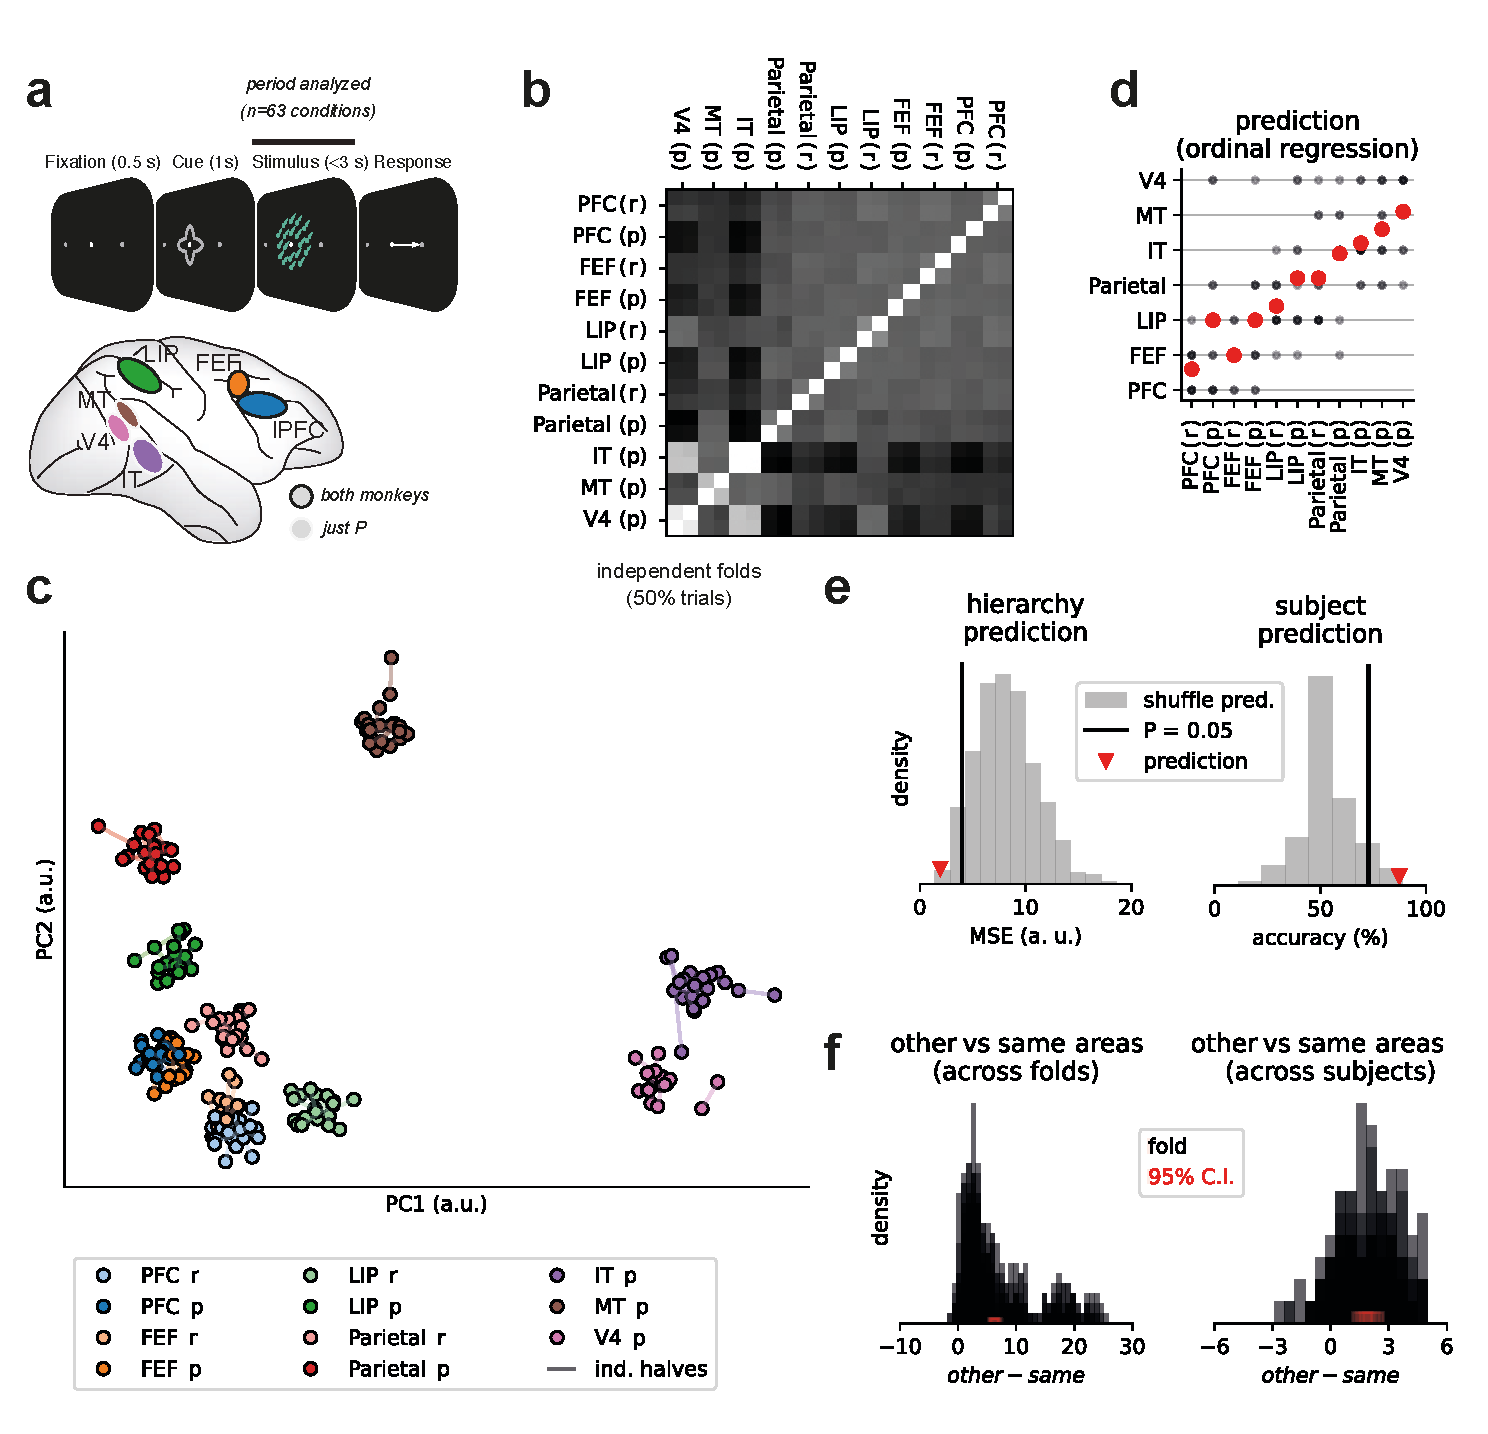
\includegraphics[scale=0.7]{content/figures/miller.pdf}
    \caption{\textbf{Regional geometry reflects anatomical hierarchy across two primates. }\textbf{a}. Description of a multi-region dataset analyzed with deterministic metric. \textbf{b.} Matrix of dissimilarities between all areas of each subject and two independent partitions. \textbf{c.} PCA visualization of B. Dark colors are from subject P and light colors from subject R. Different dots (n=10) are different repetitions of the analyses, aligned with Procrustes analyses for visualization. Independent partitions are connected by a colored line. \textbf{d.} Areas can be predicted using ordinal regression (cross-validated). Black circles mark predictions of each n=10 partitions, and red circles the average prediction. \textbf{e.} Both hierarchy and subject identity can be predicted above chance. \textbf{f.} Areas are more similar to each other than to other random areas. Left, distance calculated between independent partitions of the same area. Right, distance calculated across subjects. }
    \label{fig:miller}
\end{figure}

In a second analysis, we turned to the International Brain Laboratory Brainwide Map \parencite{angelaki2025brain} and to the encoding model fit to it by \textcite{posani2026}, in which each neuron is summarized by its time-varying coefficients for $8$ task and behavioral variables (block, stimulus side, contrast, choice, outcome, wheel, whisking and licking). Following that work, we retained neurons whose encoding model improved on a variable-agnostic null ($\Delta R^2 > 0.015$) and areas with at least $50$ such neurons, leaving $4617$ neurons across $K = 22$ cortical areas. \textcite{posani2026} average these coefficients across the neurons of an area, reducing each area to a single selectivity profile. Instead, we treated each neuron's coefficients as a tuning curve and computed pairwise Procrustes distances between the resulting populations (\hl{sup}). In addition, we subsampled every area to $50$ neurons and averaged over $20$ subsamples, and compared the result against two baselines: two disjoint halves of the same area ($d=0.60$) and a null in which area labels were shuffled across neurons ($d = 0.55$). Distances between areas exceeded both ($0.71$; \hl{p=XXX} against the shuffle). Areas that are more strongly connected anatomically had more similar geometry (Spearman $\rho = -0.51$, $p = 2\times10^{-16}$, \textit{Fig.} \ref{fig:allen}e), using the connectivity matrix of \textcite{harris2019,posani2026}. This result is essentially a replication of \textcite{posani2026}, but using a proper metric allows us to build a region space, as done with the Allen dataset (\textit{Fig.} \ref{fig:allen}a-c). Interestingly, embedding the dissimilarity matrix appeared to organize areas along a sensory-to-associative axis (\textit{Fig.} \ref{fig:allen}f). Next, we quantify this impression by doing regression in the region space: ridge regression trained on all but one area predicted the held-out area's position in the anatomical hierarchy above chance ($\rho = 0.59$, $p = 4\times10^{-3}$, \textit{Fig.} \ref{fig:allen}g.

Finally, we examined data from two nonhuman primate subjects performing a complex decision-making task (\textit{Fig.} \ref{fig:miller}a) while recording from $K=7$ regions, published in~\textcite{Siegel2015-cz}. 
Calculating pairwise shape distances between all areas and independent  partitions of the datasets for each brain region (\textit{\nameref{sec:methods}}, \textit{Fig.} \ref{fig:miller}b) revealed several interesting features that are noticeable when the dissimilarity matrix visualized in 2D (\textit{Fig.} \ref{fig:miller}c). Namely, we found that regions were organized by anatomical hierarchy, that independent partitions (connected in \textit{Fig.} \ref{fig:miller}c) were closer to each other than to other regions and that similar areas of different subjects (different shades of the same color) were more similar to each other than to other regions.
We quantified these interesting features in the following way. First, the anatomical location (Fig \ref{fig:miller}d,e) and the subject (Fig \ref{fig:miller}e, right) of individual brain regions could be predicted with threshold-based ordinal logistic regression trained and tested in independent partitions of the dissimilarity matrix (\textit{\nameref{sec:methods}}, \textit{Fig.} \ref{fig:miller}d). Second, independent partitions of the same region are more similar to each other than partitions of different regions (\textit{Fig.} \ref{fig:miller}f, left). Finally, the same areas (e.g. PFC R and PFC P) of different animals are more similar than different areas (\textit{Fig.} \ref{fig:miller}f, right).   

In sum, by using shape distances to compare neural representations across brain regions, we have recovered anatomical position in an unsupervised fashion in both mice and monkeys.
Moreover, by exploiting the metric properties of shape space we could perform both supervised and unsupervised learning methods on that space (i.e. linear regression and clustering, respectively) and rigorously quantify hypotheses developed through visual inspection (e.g. region organization by anatomical hierarchy in PCA space was quantified using regression or clustering in the full space).

